\title{Ослабленный синтаксический анализ динамически формируемых выражений на основе алгоритма GLL}

\titlerunning{Ослабленный синтаксический анализ динамически формируемых выражений на основе алгоритма GLL}

\author{Рагозина Анастасия Константиновна}

\authorrunning{А.К.Рагозина}

\tocauthor{А.К.Рагозина}
\institute{Санкт-Петербургский государственный университет\\
\email{ragozina.anastasiya@gmail.com }}

\maketitle             

\begin{abstract}
Данная работа посвящена описанию подхода к синтаксическому анализу регулярных множеств. 
Подобная задача возникает при анализе встроенных языков или же поиске соответствий в 
метагеномных сборках в задачах биоинформатики. Регулярное множество задаётся с помощью 
конечного автомата, порождающего цепочки, и нужно проверить принадлежат ли эти цепочки 
языку, задаваемому грамматикой. В качестве основы использовался алгоритм обобщённого 
синтаксического анализа GLL из-за его высокой скорости работы.
\end{abstract}

\section*{Введение}

Синтаксический анализ, как правило, используется для построения структурного представления кода с использованием грамматики, описывающей разбираемый язык. Абстрактное синтаксическое дерево, являющееся результатом работы синтаксического анализатора, в дальнейшем используется для проведения статического анализа кода или же в каких-то других целях. Как правило, на вход синтаксическому анализатору подаётся линейная последовательность токенов, представляющая код программы. Однако могут возникать ситуации, когда вход не может быть представлен линейно. Такие ситуации могут возникать, например, при автоматической генерации кода. Генерация может происходить в циклах, с использованием условных операторов или строковых операций. Поэтому для описания генерируемых цепочек можно использовать конечный автомат, порождающий цепочки, который уже не будет являться линейным. Такую задачу будем называть синтаксическим анализом регулярных множеств.

Кроме этого, ещё одной областью, где может быть применим синтаксический анализ регулярных множеств, является бионформатика. Одной из часто возникающих задач в биоинформатике является классификация организмов, находящихся в образцах, полученных из окружающей среды~\cite{bioRNA}. По образцам строится метагеномная сборка, которая содержит в себе смесь из ДНК всех содержащихся в сборке организмов. В свою очередь ДНК является последовательностью символов в алфавите \{A, C, G, T\}. ДНК организмов, которые относятся к одному и тому же виду, содержат одинаковые подцепочки, которые и необходимо выделить, чтобы классифицировать организм. Как правило, эти подцепочки~--- это последовательности РНК. РНК может быть описана с помощью грамматики. Метагеномная сборка, в свою очередь, может быть представлена в виде графа с цепочками на рёбрах. Таким образом, в таком графе необходимо найти цепочки, выводимые в грамматике, описывающей РНК. 

Грамматики, описывающие структуру РНК, являются неоднозначными. Грамматика называется неоднозначной, если одна и та же цепочка может быть выведена несколькими способами. Такие алгоритмы синтаксического анализа как LR и LL не позволяют обрабатывать неоднозначные грамматики. Для работы с неоднозначными грамматиками существуют алгоритмы обобщённого синтаксического анализа GLR~\cite{GLR}, GLL~\cite{GLL}. В рамках проекта YaccConstructor~\cite{YaccConstructorPage, YaccConstructorPaper} был реализован алгоритм GLL, кроме того, была предложена его модификация для обработки нелинейных входных данных~--- графов. Реализованная модификация позволяет находить цепочки транспортной РНК (тРНК) в небольших метагеномных сборках, возвращая координаты начала и конца найденной цепочки. Проблема заключается в том, что грамматика для описания тРНК является сильно неоднозначной, что сказывается на производительности и точности полученных результатов. Для повышения точности можно применять конъюнктивные грамматики~\cite{ConjGrammars}, в которых для описания продукций используется операция конъюнкции. Такие грамматики расширяют класс контекстно-свободных языков и позволяют точнее описать структуру тРНК. Данная работа посвящена описанию модификаций решения на основе алгоритма GLL для работы с конъюнктивными грамматиками.

\section{Постановка задачи}
Целью данной работы является исследование применимости символьных конечных преобразователей для лексического анализа. Для ее достижения поставлены следующие задачи:

\begin{itemize}
    \item Изучить возможности библиотеки Microsoft.Automata.
\item Провести сравнение производительности алгоритма операции композиции над символьными конечными преобразователями в библиотеке Microsoft.Automata с производительностью операции композиции над конечными преобразователями в исследовательском проекте YaccConstructor.
\item На основании полученных результатов сделать выводы о применимости библиотеки Microsoft.Automata для лексического анализа в проекте YaccConstructor.
  \end{itemize}

\section{Обзор}
\lstset{basicstyle=\normalsize\ttfamily, columns=fullflexible}
В данном обзоре рассматриваются некоторые подходы к заданию принтеров и форматеров, а также плагин Grammar-Kit для IntelliJ IDEA, позволяющий по БНФ-грамматике задавать синтаксический анализатор целевого языка.
Используемые плагином грамматики рассматриваются на примере грамматики языка While \cite{paper:nielson}.

\subsection{Подходы к заданию принтеров и форматеров}
Рассмотрим некоторые подходы к заданию принтеров и форматеров.
\subsubsection{Задание форматеров по описанию синтаксиса}%Язык описания синтаксиса}
Существуют различные подходы к заданию принтеров для целевого языка.
Один из них описан в \cite{paper:tbe}.
Авторы предлагают язык описания синтаксиса, по которому можно получить и синтаксический анализатор, и принтер для языка.
Описание синтаксиса состоит из правил, которые схожи с правилами формальных грамматик, но которые также задают и стиль форматирования для данной структуры языка.
Приведенное ниже правило вывода описывает основные арифметические выражения:
{
    \lstinputlisting{codes/tbeif.txt}
    %% =================================================
    %% ПРИМЕР ПОИНТЕРЕСНЕЕ
    %% непонятно, как задаются условия форматирования
    %% =================================================
}
\noindent
Первое преобразование определяет шаблон для выражений, состоящих из чисел.
Остальные преобразования задают шаблоны для операций сложения и вычитания.
Каждое из них состоит из двух меток \lstinline{<Exp>} для подстановки выражений, арифметического знака, а также двух пробелов вокруг этого знака.
Само правило явно задает способ, которым будут отформатированы арифметические выражения полученного языка.
%При дальнейшем форматировании программ на данном языке, арифметические выражения будут иметь вид, задаваемый правилом.
Вместо пробелов можно также указать табуляции и/или переносы строк.
Недостатком данного подхода является то, что правила форматирования задаются заранее, и, чтобы их изменить, необходимо менять описание синтаксиса языка.
Кроме того, каждое такое правило задает единственный вариант форматирования данной структуры.

%\subsubsection{}
Наиболее близкий к нашей работе метод описан в \cite{paper:asf-sdf}.
Принтер языка может быть получен по ASF+SDF описанию языка \cite{paper:klint}, что представляет собой контекстно-свободную грамматику.
При этом правила форматирования не указываются.
Недостатком данного подхода является то, что при генерации принтера задается базовый стиль форматирования, и, чтобы его изменить, необходимо редактировать сгенерированный код, тогда как подход с использованием синтаксических шаблонов позволяет пользователю декларативным образом настраивать принтер.

\subsubsection{Форматеры, встроенные в IDE}
Так же широко распространены форматеры, встроенные в IDE.
Они используют множество настроек для задания стиля форматирования (рис.~\ref{ov:settings}).
Среди них: тип и размер отступов, расположение фигурных скобок в C-подобных языках, политика переноса списочных выражений на новую строку и десятки других.
Набор этих настроек выбирается разработчиком форматера на основе его представлений о возможных стилях кодирования для целевого языка.
Такие форматеры обычно тесно интегрированы с IDE, имеют высокую скорость работы, и их выразительности, как правило, достаточно для задания необходимого стиля форматирования.
Однако для поддержки нового языка необходимо определить нужный набор настроек и вручную реализовать форматер.
В случае, если пользователю необходимо придерживаться стиля кодирования некоторой существующей кодовой базы, то ему нужно самостоятельно определить значения этих настроек.
Данный недостаток отсутствует в работе \cite{paper:sformatters}, где авторы предлагают инструмент, позволяющий получить некоторые настройки форматера из существующего программного кода.
Недостатком подхода является то, что число этих настроек невелико: система позволяет определять только стиль отступов, стили именования идентификаторов, необходимое количество комментариев.
Другой подход \cite{blog:genformat} предлагает использование генетического алгоритма 
%\footnote{\texttt{https://en.wikipedia.org/wiki/Genetic\textunderscore algorithm}} 
для поиска настроек форматера в исходном коде программ на языке C.

%и в работе\footnote{\texttt{https://blog.jetbrains.com/clion/2015/11/applying-genetic-algorithms-to-automatic-code-formatting/}}. 
%Они представляют собой способы автоматического вычленения настроек форматирования из программного кода.
\begin{figure}[t]
    \centering
    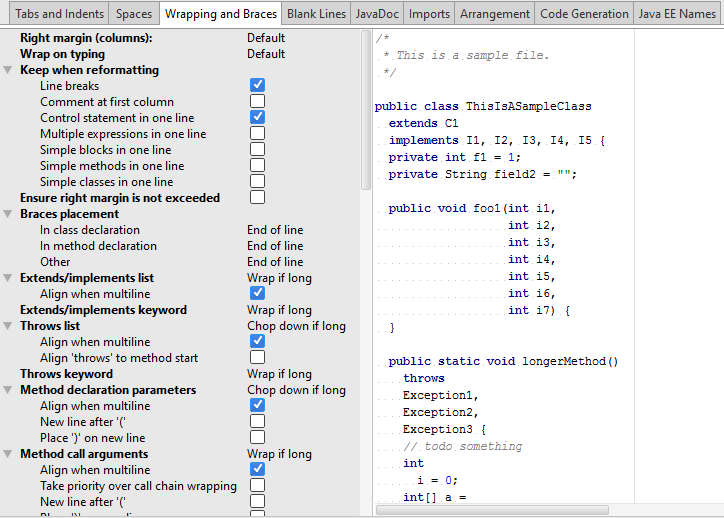
\includegraphics[width=.7\textwidth]{images/settingsjava.PNG}
    \caption{Настройки форматера языка Java в IntelliJ IDEA}
    \label{ov:settings}
\end{figure}

\subsection{Grammar-Kit}
Как уже было отмечено, для поддержки нового языка в платформе IntelliJ IDEA необходимо разработать синтаксический анализатор.
Для его генерации можно использовать плагин Grammar-Kit.
В качестве системы описания синтаксиса языка используется БНФ-грамматика.
Результатом работы плагина является код синтаксического анализатора и иерархия классов внутреннего представления. %(для IntelliJ IDEA~--- \emph{PSI-классов}).%PSI-классов.
%PSI-классом является каждая структура языка, вместе они образуют иерархию.

%Кроме того, при реализации поддержки нового языка в платформе возникает потребность в форматере.
%Мы хотим задавать принтер для языка, используя его грамматику.
% что тут еще описывать?
%\subsection{Грамматика языка While}
%Для апробации метода, описанного в \cite{paper:while}, использовался язык While, поэтому будем рассматривать грамматики, с которыми работает Grammar-Kit, на примере грамматики языка While.
Рассмотрим грамматику языка While, для которого производилась апробация метода, описанного в \cite{paper:while}.
%Рассмотрим БНФ-грамматику, использующуюся в плагине Grammar-Kit на примере грамматики языка While (рис.~\ref{ov:whileBnfFull}).
%\begin{figure}[p]
%\fvset{frame=lines,framesep=5pt}
While~--- язык программирования, содержащий следующие конструкции: чтение из стандартного потока (\lstinline{read}) и запись в стандартный поток (\lstinline{write}), оператор ветвления (\lstinline{if}), цикл с предусловием (\lstinline{while}); процедуры (\lstinline{proc}), бинарные выражения (\lstinline{binary_expr}), в том числе булевы (\lstinline{binary_bexpr}) и т. д.
% (рис.~\ref{ov:whileI},~\ref{ov:whileII},~\ref{ov:whileIII}).
\begin{figure}[h]
 %   \begin{pyglist}[numbers=left,numbersep=5pt]%, basicstyle=\ttfamily]
    \begin{lstlisting}[numbers=left, numbersep=3pt, basicstyle=\ttfamily\small, numberstyle=\tiny, frame=bottom, language={}]
whileFile  ::= proc_list stmt_list
stmt_list  ::= stmt*
proc_list  ::= procedure*
stmt       ::= skip|assign|if|while|write|read
skip       ::= 'skip' ';'
write      ::= 'write' '(' expr ')' ';'
read       ::= 'read' '(' id ')' ';'
assign     ::= id ':=' expr ';'
if         ::= 'if' '(' bexpr ')' 'then' stmt_list ('else' stmt_list)? 'fi'
while      ::= 'while' '(' bexpr ')' 'do' stmt_list 'od'
procedure  ::= 'proc' id '(' param_list ')' stmt_list 'endp'
param_list ::= ref_expr? (',' ref_expr)*
...
 \end{lstlisting}
    \caption{Грамматики языка While. Операторы языка}
    \label{ov:whileI}
\end{figure}
\noindent
На рис.~\ref{ov:whileI} представлена часть грамматики языка While, задающая множество операторов.
Рассмотрим правило грамматики, задающее оператор ветвления.
Правая часть правила состоит из терминалов \lstinline{'if'}, \lstinline{'then'} \lstinline{'('} и др.; нетерминалов: \lstinline{bexpr}, \lstinline{stmt_list}, а также условного вхождения \lstinline{('else' stmt_list)?} (то есть конструкция может отсутствовать в программах на данном языке).
Некоторые правила грамматики имеют модификаторы, которые используются для дополнительных указаний генератору синтаксического анализатора (рис.~\ref{ov:whileII}).
\begin{figure}[h]
    %\begin{pyglist}[numbers=left,numbersep=5pt]
    \begin{lstlisting}[numbers=left, numbersep=3pt, basicstyle=\ttfamily\small, numberstyle=\tiny, frame=bottom, language={}]
...
fake ar_op        ::= plus_op|mul_op
fake binary_expr  ::= expr ar_op expr 

expr              ::= factor plus_expr *
left plus_expr    ::= plus_op factor
plus_op           ::= '+'|'-'
private factor    ::= primary mul_expr *
left mul_expr     ::= mul_op primary
mul_op            ::= '*'|'/'|'%'
private primary   ::= literal_expr | ref_expr | paren_expr
paren_expr        ::= '(' expr ')'
ref_expr          ::= id
literal_expr      ::= number

fake bl_op        ::= or|and
fake binary_bexpr ::= bexpr bl_op bexpr
...
    \end{lstlisting}
    %\end{pyglist}
    \caption{Грамматика языка While. Выражения с модификаторами}%?
    \label{ov:whileII}
\end{figure}
\noindent
Модификатор \lstinline{fake} указывает системе, что не нужно генерировать код синтаксического анализатора для обработки данной структуры, однако генерируется иерархия классов внутреннего представления, \lstinline{private} указывает, что не будет сгенерирована иерархия классов, \lstinline{left} используется для поддержки левоассоциативности, а также некоторые другие\footnote{Посмотреть полный список можно по адресу \texttt{https://github.com/JetBrains/Grammar-Kit}}.
Модификатор \lstinline{private} используется для правил грамматики, которые не имеют представления в синтаксическом дереве.
Среди них те, которые используются для устранения левой рекурсии.
%которые не влияют на синтаксис языка, например, такие, которые используются для устранения левой рекурсии.
Например, на рис.~\ref{ov:whileExpr} представлено описание правил с рис.~\ref{ov:whileII} (строки 5--14), но в более естественной для человеческого восприятия леворекурсивной форме.
\begin{figure}[h]
    %\lstinputlisting{codes/whileExpr.txt}
    %\begin{pyglist}[numbers=left,numbersep=5pt]
    \begin{lstlisting}[numbers=left, numbersep=3pt, basicstyle=\ttfamily\small, numberstyle=\tiny, frame=bottom, language={}]
expr         ::= plus_expr | mul_expr | paren_expr | ref_expr | literal_expr
plus_expr    ::= expr plus_op expr
plus_op      ::= '+'|'-'
mul_expr     ::= expr mul_op expr
mul_op       ::= '*'|'/'|'%'
paren_expr   ::= '(' expr ')'
ref_expr     ::= id
literal_expr ::= number
    \end{lstlisting}
    %\end{pyglist}
    \caption{Грамматики языка While. Выражения в естественной леворекурсивной форме}
    \label{ov:whileExpr}
\end{figure}
\noindent
Однако грамматика, с которой работает Grammar-Kit, не должна содержать леворекурсивных правил.
Устраняя левую рекурсию, мы получим описание выражений на рис.~\ref{ov:whileII} (строки 5--14).
Кроме того, появляются новые правила, которые с точки зрения синтаксического анализа (а следовательно, и форматирования) являются избыточными.
В данном случае такими являются \lstinline{factor} и \lstinline{primary} на рис.~\ref{ov:whileII}.
\begin{figure}[b]
    %\begin{pyglist}
    \begin{lstlisting}[numbers=left, numbersep=3pt, basicstyle=\ttfamily\small, numberstyle=\tiny, frame=bottom, language={}]
{   parserClass="com.intellij.whileLang.parser.WhileParser"
    psiClassPrefix="Psi"
    psiImplClassSuffix="Impl"
    psiPackage="com.intellij.whileLang.psi.impl"
    tokens=[...]
    ...
}
...
    \end{lstlisting}
    %\end{pyglist}
    \caption{Заголовок файла с грамматикой}
    \label{ov:whileIII}
\end{figure}
% про left
Каждый файл с грамматикой языка содержит в себе заголовок, в котором описывается различная дополнительная информация: используемые в сгенерированных файлах классы, префиксы и суффиксы сгенерированных классов внутреннего представления, Java-пакеты, множество терминальных символов грамматики (\emph{tokens}) и др. (см рис.~\ref{ov:whileIII}).





\section{Алгоритм анализа регулярных множеств}
Целью данной работы является создание алгоритма синтаксического анализа регулярных множеств, который может быть применим для анализа встроенных языков. Как упоминалось ранее, встроенный код порождается в момент выполнения основной программы. Для генерации могут использоваться строковые операторы, условные операторы и циклы из-за чего такой код не может быть представлен линейно. Результатом работы лексического анализатора на таком коде является не линейный поток токенов, а конечный автомат над алфавитом токенов. В рамках данной работы на такие автоматы накладывается следующее ограничение: они должны быть детерминированными. Если это условие не будет выполняться, то нельзя будет однозначно выбрать, по какому пути производить разбор. Например, для встроенного кода на листинге~\ref{lst:brExpr} будет построен конечный автомат на рис.~\ref{input}.

%\fvset{frame=lines,framesep=5pt}
\begin{listing}
\begin{pyglist}[language=csharp,numbers=left,numbersep=5pt]
 string expr = "" ;
 for(int i = 0; i < len; i++) 
 {
     expr = "()" + expr;
 }
\end{pyglist}
\caption{Код на C\#, динамически формирующий скобочную последовательность}
\label{lst:brExpr}
\end{listing}

\begin{figure}[h]
 \centering
 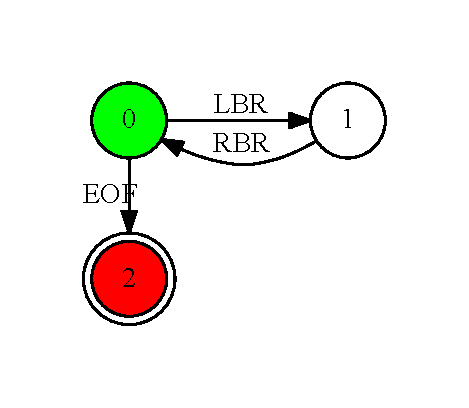
\includegraphics[width=0.3\textwidth]{Ragozina/pics/input.pdf}
 \caption{Конечный автомат, представляющий аппроксимацию встроенного кода для листинга~\ref{lst:brExpr} }
 \label{input}
\end{figure}

В алгоритме вместо хранения позиции во входном потоке теперь хранится номер вершины во входном графе. Поскольку вход является нелинейным, то вместо того, чтобы просматривать один текущий входной символ на каждом шаге, рассматриваются все исходящие рёбра для текущей вершины и выбирается одно (как упоминалось ранее, автомат детерминирован, поэтому это возможно), соответствующее текущему терминальному символу в грамматике. Если такого ребра нет, то алгоритм просто продолжает свою работу --- из очереди достаётся новый дескриптор и процесс возобновляется. 

Для автоматического создания синтаксических анализаторов существует несколько подходов. В рамках первого подхода весь код парсера генерируется по грамматике. Чаще всего такой подход используется при генерации анализаторов, построенных методом рекурсивного спуска. При генерации нисходящих анализаторов для каждого нетерминала генерируются функции, которые последовательно вызываются в процессе разбора. Несмотря на то, что нисходящие анализаторы просты для разработки, и поэтому чаще всего создаются вручную, существуют инструменты для автоматической генерации таких анализаторов. Например, инструмент ANTLR~\cite{antlr} --- генератор парсеров, позволяющий автоматически создавать анализаторы на одном из целевых языков программирования по описанию LL(*)-грамматики на языке, близком к EBNF. Структура генераторов такого типа изображена на рис.~\ref{genTypes}{\it (а)}.

\begin{figure}
 \centering
 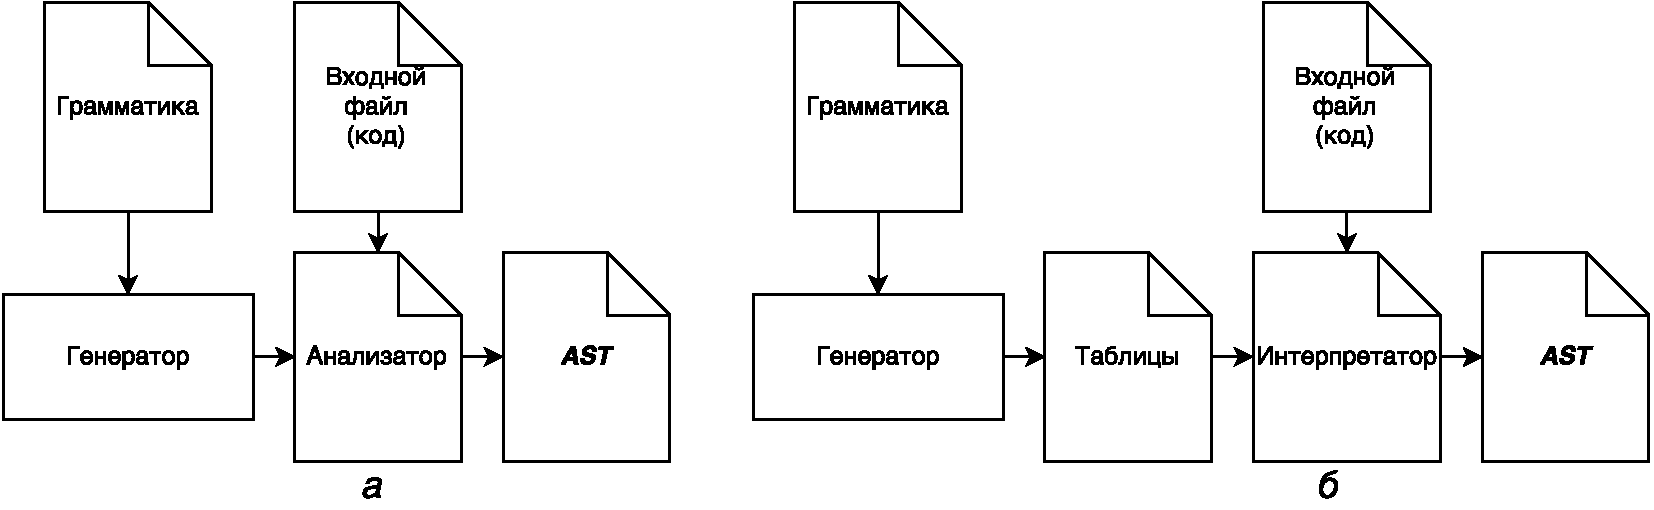
\includegraphics[width=\textwidth]{Ragozina/pics/GeneratorTypes.pdf}
 \caption{Подходы к генерации синтаксических анализаторов}
 \label{genTypes}
\end{figure}

Существует ещё один подход для генерации синтаксических анализаторов, который используется для получения табличных анализаторов. Отдельно создаётся интерпретатор, который содержит в себе основную логику алгоритма. Интерпретатор пишется вручную и переиспользуется. По грамматике каждый раз генерируется дополнительная информация, которая необходима интерпретатору в процессе работы. Структура такого генератора представлена на рис.~\ref{genTypes}{\it (б)}. Чаще всего в качестве дополнительной информации генерируются таблицы синтаксического анализа, управляющие процессом разбора.

В оригинальных работах, описывающих GLL-алгоритм, используется первый подход. В рамках данной работы был выбран второй подход из-за его гибкости и универсальности. Вместо генерации функций по слотам грамматики и их последовательного вызова, в главном цикле алгоритма просто рассматриваются все возможные состояния, в которых может находиться парсер. В зависимости от того, какой символ во входном потоке и какая позиция в грамматике, в процессе разбора рассматриваются следующие ситуации.

\begin{itemize}
\item Если текущий символ в грамматике является терминалом $x$ и существует исходящее из текущей вершины ребро, помеченное этим нетерминалом, то указатель в грамматике нужно сдвинуть на одну позицию вправо, $x \rightarrow \alpha X \cdot \beta$, и текущей вершиной назначить конечную вершину ребра. Никаких дополнительных действий со стеком при этом не производится. Иначе, если нет ребра, помеченного терминалом $х$, то текущая ветка разбора считается ошибочной, отбрасывается и  разбор продолжается с использованием следующего дескриптора.
\item Если текущий символ в грамматике является нетерминалом $a$, то необходимо в стек записать слот, по которому продолжить разбор после того, как правило для $a$ будет разобрано. Указатель в грамматике перемещается на $a \rightarrow \cdot \gamma $, а номер вершины во входном потоке остаётся без изменений.
\item Если указатель в грамматике имеет следующий вид $x \rightarrow \alpha\cdot$ и стек не пуст, то слот вида $y \rightarrow \delta x \cdot \mu$, который хранится в этот момент в текущей вершине стека, извлекается и становится текущим.
\item Если текущий слот имеет вид $s \rightarrow \tau\cdot$, и весь входной поток рассмотрен, то разбор завершается успешно, иначе разбор заканчивается ошибкой. В случае успешного завершения разбора возвращается дерево, иначе сообщение об ошибке.
\end{itemize}

Наличие циклов во входном графе никак не влияет на процесс разбора. Дескрипторы позволяют без каких-либо изменений процесса разбора обработать их. Это делает результирующий алгоритм более простым в отличие от алгоритма, основанного на RNGLR , в который потребовалось внести существенные изменения для поддержки циклов~\cite{RelaxedARNGLR}. За счёт того, что каждый раз при добавлении дескриптора выполняется проверка всей четвёрки целиком (позиция во входе, слот, вершина стека и часть леса разбора), то лишние дескрипторы с одинаковыми деревьями не создаются. Переиспользование уже созданных узлов также позволяет избежать создания лишних деревьев: если дерево с определёнными координатами и соответствующим правилом вывода уже было создано, то повторно такое дерево создаваться не будет.

В алгоритме так же поддерживается четвёрка: слот (вместо имени функции), номер вершины в графе, вершина стека и узел дерева. Поскольку вызов функций заменён на обработку ситуаций, возникающих в процессе анализа, в теле основной функции, то появилась необходимость определять, какое правило вывода использовать для разбора. Для определения правила используются LL-таблицы, где в каждой ячейке может быть несколько правил для разбора, что соответствует ситуации наличия в грамматике неоднозначностей. Анализатор состоит из функции, содержащей основной цикл алгоритма, функции управляющей процессом разбора и функций для построения дерева и стека.

\begin{listing}[H]
\hrule
\begin{algorithmic}
\caption{Функция, содержащая в себе основную логику алгоритма}
\label{parsing}
\Function{parsing()}{}
	\State{$condition \gets true$}
	\If{$isEpsilonRule(cL.rule)$} 
		\State{$cR \gets$ $new TerminalNode("Epsilon", packExtension (cI, cI))$}
		\State{$cN \gets$ $getNodeP(cL, cN, cR)$}
		\State{$pop(cU, cI, cN)$}
    \Else
		\If{$isEndOfRule(cL.rule, cL.position)$}
			\State{$curSmb \gets$ $grammarRules[cL.rule][cL.position]$}
			\If{$isTerminal(curSmb)$}
				\State{$curSmb \gets$ $grammarRules[cL.rule][cL.position]$}
				\If{$cI.OutEdges$ contains edge labeled with $curSmb$}
					\State{$curEdge \gets$ edge labeled with $curSmb$}
					\State{$cR \gets$ $getNodeT(curEdge)$}
					\State{$cI \gets$ $curEdge.TargetVertex$}
					\State{$cL \gets$ $label(cL.rule, cL.position + 1)$}
					\State{$cN \gets$ $getNodeP(cL, cN, cR)$}
				    \State{$condition \gets$ $false$}
				\EndIf
			\Else
				\State{$cU \gets$ $create(cI, label(cL.rule, cL.position + 1), cU, cN)$}
				\ForAll{$edge$ in outgoing edges of $cI$}
					\ForAll{$rule in table[curSymbol, edge.Token]$}
						\State{$addContext(cI, packLabel(rule, 0), cU, \$)$}
					\EndFor
				\EndFor	
			\EndIf
		\Else
		    \State{$pop(cU, cI, cN)$}
		\EndIf
    \EndIf
\EndFunction
\end{algorithmic}

\hrule
\end{listing}

\begin{listing}
\hrule
\begin{algorithmic}
\caption{Функции, управляющие процессом разбора }
\label{control}
\Function{control()}{}
	\State{$condition \gets$ $true$}
	\While{not $stopr$}
		\If{$condition$} {$dispatcher()$}
		\Else {$processing()$} 
		\EndIf
	\EndWhile
\EndFunction

\Function{dispatcher()}{}
	\If{$\mathcal{Q}$ is not empty} 
		\State{$currentContext \gets$ $\mathcal{R}.Dequeue()$}
		\State{$cI \gets$ $currentContext.Index$}
		\State{$cU \gets$ $currentContext.GSSNode$}
		\State{$cL \gets$ $currentContext.Label$}
		\State{$cN \gets$ $currentContext.SPPFNode$}
		\State{$cR \gets$ $DummySPPFNode$}
		\State{$condition \gets$ $false$}
    \Else
		\State{$stop \gets$ $true$}
    \EndIf
\EndFunction
\end{algorithmic}
\hrule
\end{listing}

На листинге~\ref{control} приведены две функции управляющие разбором. Функция \texttt{control()} в зависимости от значений булевых переменных \texttt{stop} и \texttt{condition} вызывает функции \texttt{dispatcher()} или \texttt{parsing()}. Функция \texttt{dispatcher()} извлекает из очереди дескриптор, присваивает значения переменным. Функция \texttt{parsing()} на листинге~\ref{parsing} содержит в себе основную логику алгоритма.


\subsection{Пример работы алгоритма}
Рассмотрим следующий пример. В качестве входных данных будем испоьзовать конечный автомат $M$, представленный на рис.~\ref{InputGraph}, который генерирует произвольные скобочные последовательности. Необходимо построить лес разбора для всех цепочек, порождаемых автоматом $M$, выводимых в грамматике $G_4$ (листинг~\ref{grmG4}), описывающей язык правильных скобочных последовательностей.
\begin{listing}
\caption{Грамматика $G_4$}
\label{grmG4}
\centering
$\begin{array}{rl}
s \rightarrow LBR \ s \ RBR \ s \ \varepsilon \  | \ \varepsilon 
\end{array}$
\end{listing}

\begin{figure}
 \centering
 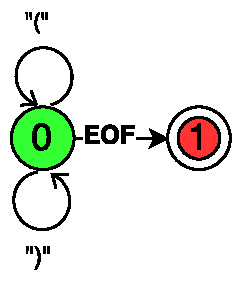
\includegraphics[width=0.3\textwidth]{Ragozina/pics/ExampleInputGraph.pdf}
 \caption{Конечный автомат, подаваемый на вход анализатору }
 \label{InputGraph}
\end{figure}

В результате работы описанного алгоритма построено сжатое представление леса разбора, представленное на рис.~\ref{ExSppf}. Циклы в сжатом представлении леса разбора отображают наличие циклов во входном конечном автомате и позволяют извлекать потенциально бесконечное множество деревьев, каждое из которых соответствует цепочке, порождаемой автоматом.

\begin{figure}
 \centering
 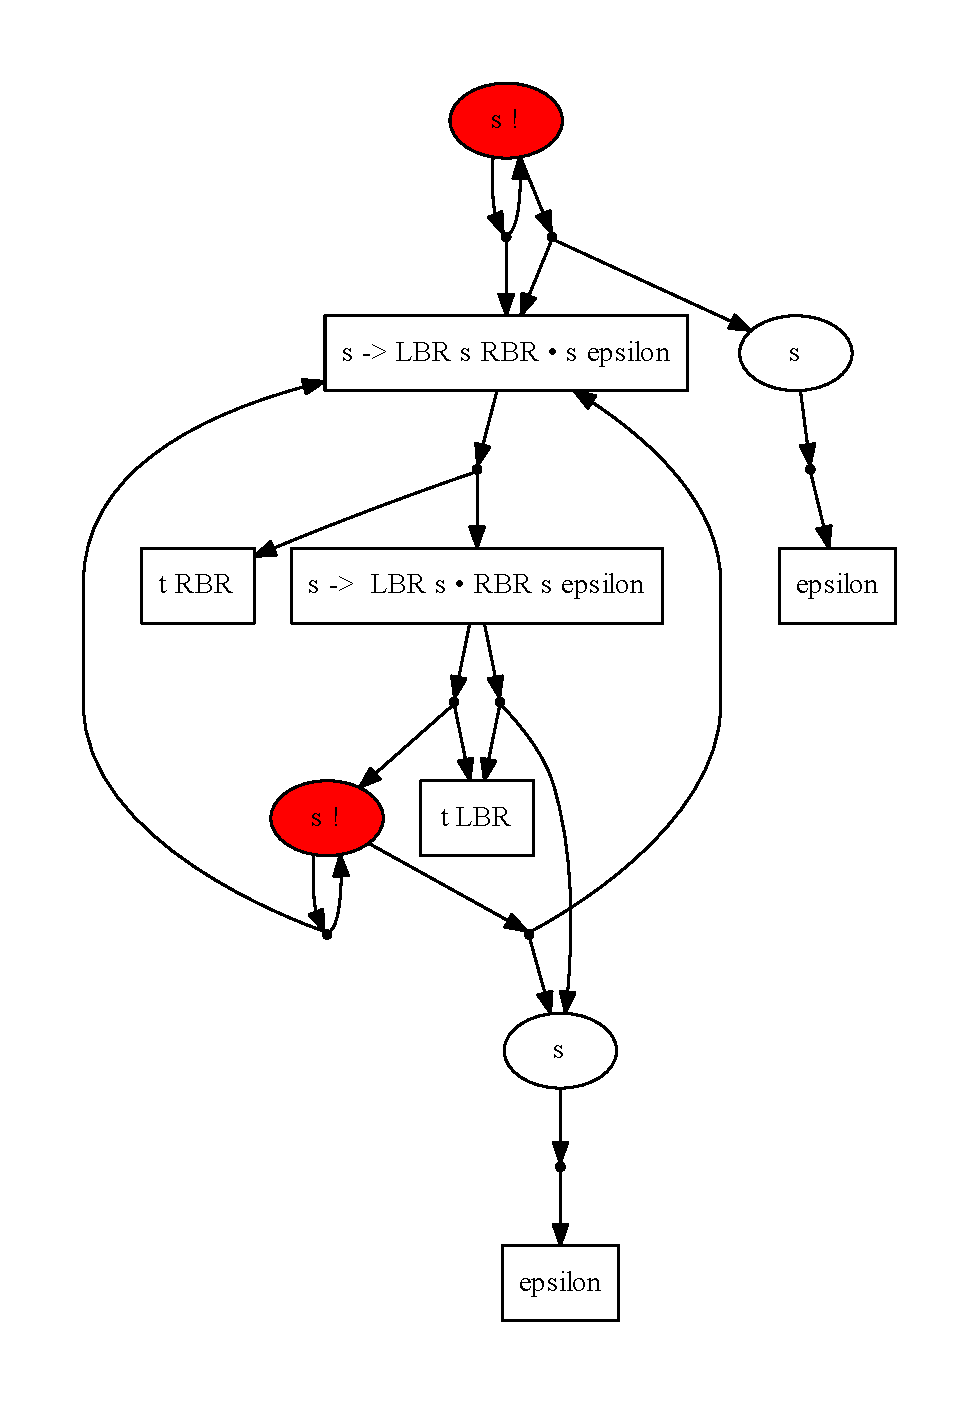
\includegraphics[width=\textwidth]{Ragozina/pics/SppfExample.pdf}
 \caption{Сжатое представление леса разбора для грамматики $G_4$ и конечного автомата на рис.~\ref{InputGraph} }
 \label{ExSppf}
\end{figure}

\subsection{Доказательство корректности}
Для того чтобы показать, что предложенный алгоритм работает корректно сначала нужно доказать, что процесс останавливается.

\textsc{Теорема 1.} 
\textit{Алгоритм завершает свою работу для произвольного детерминированного конечного автомата и контекстно-свободной грамматики.}

\textsc{Доказательство.}

Алгоритм завершает свою работу как только очередь дескрипторов становится пустой. Дескриптор с определённым набором значений полей в очередь добавляется лишь единожды. Таким образом, чтобы показать завершаемость алгоритма достаточно доказать, что количество дескрипторов конечно. 

Дескриптор состоит из четырёх элементов --- слот, индекс во входном потоке, вершина стека, дерево. Таким образом, общее количество дескрипторов не превышает прямого произведения возможного количества каждого из этих элементов. Количество индексов не больше количества вершин входного графа. Количество слотов конечно, потому что грамматика конечна. Вершина стека определяется парой --- слот и индекс, и значит тоже конечно. Часть леса, хранимая в дескрипторе, определяется однозначно именем нетерминала или слотом и двумя координатами во входном графе. Обе составляющие конечны. $\square$

Таким образом было показано, что количество дескрипторов --- конечное число.

\textsc{Определение 1.} 
\emph{Корректное дерево}~--- это упорядоченное дерево со следующими свойствами.
\begin{enumerate}
  \item Корень дерева соответствует стартовому нетерминалу грамматики $G$.
  \item Листья соответствуют терминалам грамматики $G$. Упорядоченная последовательность листьев соответствует некоторому пути во входном графе.
  \item Внутренние узлы соответствуют нетерминалам грамматики $G$. Потомки внутреннего узла (для нетерминала $N$) соответствуют символам правой части некоторой продукции для $N$ в грамматике $G$.
\end{enumerate}

Для того, чтобы доказать, что SPPF содержит только корректные деревья, сначала необходимо доказать следующую лемму.

\textsc{Лемма 1.} 
\textit{Для любой части леса $t$, построенного в процессе вывода, существует путь в графе $р$, такой что крона $t$ покрывает этот путь. }

\textsc{Доказательство.}

Для доказательство используется индукция по построению SPPF. 

\textsc{База.}

Для терминальных узлов утверждение очевидно. Терминальный узел соответствует ровно одному ребру во входном графе и строится только после прохода по этому ребру. Построение эпсилон узлов никак не зависит от входного графа, а производится только в соответствии с грамматикой. 

\textsc{Переход.}

Достаточно доказать для упакованных ячеек, всё остальное доказывается аналогично. Создание упакованных ячеек происходит в двух случаях --- при чтении нового терминала из входного потока или изъятии вершины стека, что значит, что текущий нетерминал был разобран и необходимо вернуться к точке, с которой этот разбор начался. 

Рассмотрим первый случай. У нас есть часть леса, которая соответствует какому-то пути $p$ в графе от вершины $v_0$ до $v_1$. Текущая позиция во входном потоке соответствует правой координате для этой части SPPF. При считывании нового терминала, создаётся упакованная ячейка, левым сыном которой становится уже построенная часть SPPF, а правым --- терминал. Получаем новую часть леса, соответствующее пути $P_1 = v_0 \dots v_1 v_{1+1}$.

Рассмотрим второй случай --- изъятие вершины со стека. Первая часть леса разбора Т1 хранится на ребре стека. Вторая часть Т2 построена по только что разобранному правилу. Каждая из этих частей соответствует какому-то подпути в графе и необходимо показать, что правая координата T1 совпадает с левой координатой T2. Это соответствует тому факту, что объединение этих частей леса даст часть леса, покрывающую путь в графе без дыр, то есть если в графе была цепочка {\it ``abcd''} и T1 соответствует {\it ``ab''}, то T2 будет соответствовать {\it ``bc''}. Для того, чтобы показать, что это условие выполняется, достаточно рассмотреть, как происходит процесс разбора. Как только в процессе обхода грамматики (в слоте) встречается нетерминал, создаётся новая вершина стека, которая хранит в себе слот с позицией за этим нетерминалом, на ребре хранится уже построенная часть леса. Правая координата этой части SPPF является номером вершины, с которой будет происходить дальнейший разбор, это число и записывается в новый дескриптор. Таким образом, после того, как нетерминал будет разобран до конца, будет создан новый упакованный узел, в котором в качестве левого потомка будет часть леса с ребра, а в качестве правого --- нетерминальный узел, левая координата которого совпадает с правой координатой левой части леса, так как именно с того места и начался разбор этого нетерминала. $\square$

Таким образом для упакованных узлов в дереве доказали необходимое. Доказательство для остальных видов узлов проводится аналогично.

\textsc{Теорема 2.} 
\textit{Любое дерево, извлечённое из SPPF, является корректным.}

\textsc{Доказательство.}

Рассмотрим произвольное извлечённое из SPPF дерево и докажем, что оно удовлетворяет определению. Первый и третий пункт определения корректного дерева следует из определения SPPF. 

Второй пункт следует из Леммы 1. Необходимо только показать, что такой путь начинается в начальной вершине и заканчивается в конечной. Действительно, так как работа алгоритма может быть начата только из начальной вершины, то левой координатой для неё будет стартовая вершина. Результатом работы алгоритма является SPPF. Узел помечается, как результирующий, если он помечен стартовым нетерминалом и его левая координата является стартовой вершиной, а правая --- финальной. $\square$

\textsc{Теорема 3.} 
\textit{Пусть грамматика Г порождает язык $L$. Тогда для каждого пути в графе $p$, соответствующего строке s из $L$, из SPPF может быть изъято корректное дерево.}

\textsc{Доказательство.}

Необходимо доказать, что SPPF содержит все корректные деревья вывода для всех корректных цепочек из входа. Как только процесс разбора начинается, в очередь дескрипторов добавляются дескрипторы для всех альтернатив стартового правила, соответствующие терминалу во входном потоке. Аналогичная ситуация происходит, как только в грамматике встречается нетерминал. Рассматриваются все альтернативы нетерминала и добавляются те, по которым может быть продолжен синтаксический анализ в соответствии со входным символом. Это гарантирует, что все альтернативы в выводе будут рассмотрены. При этом во входном графе все пути, соответствующие входным цепочкам, тоже рассматриваются, так как переход по ребру осуществляется всегда, если оно продолжает корректный префикс.$\square$

\subsection{Анализ данных большого объёма}
Одной из задач, сформулированных в данной работе, является использование предложенного алгоритма для анализа больших данных. Это востребовано, например, в задачах биоинформатики. Прежде чем формулировать задачу, следует ввести основные определения.

Исследование геномов является одной из распространённых задач биоинформатики. Информацию, содержащуюся в геноме можно представить в виде последовательностей символов и в дальнейшем эти последовательности анализировать. Геномы извлекаются из ДНК и позволяют характеризовать тот или иной организм. Для этого из генома необходимо выделить определённые участки, позволяющие сделать выводы о его свойствах. Геном (последовательность ДНК) --- строка в алфавите $\{A, C, G, T\}$, однозначно определяющая организм (или штамм), к которому она относится. Сборка --- набор подстрок генома, длина которых на порядки меньше длины самого генома. Метагеномная сборка --- смесь сборок нескольких геномов, то есть набор небольших подстрок нескольких геномов. Поскольку геном состоит из повторяющихся участков, то его можно представить в виде конечного автомата с последовательностями символов на рёбрах, который на практике часто представляется в виде графа  Де Брауна~\cite{Bruijn}.

Как упоминалось ранее, для решения задач, возникающих в биоинформатике, не нужно структурное представление вывода. Это значит, что дерево разбора, которое является результатом работы синтаксического анализатора, не нужно. Нужно лишь ответить на вопрос: порождает ли входной автомат данную подстроку или нет и вернуть координаты участка, на котором это происходит. При этом геном можно описать с помощью грамматики, т.е. про подцепочки, порождаемые входным конечным автоматом, известно, что они описываются некоторой грамматикой. Необходимо найти подавтоматы, принимающие цепочки, задаваемые некоторой грамматикой. Таким образом, предложенный алгоритм необходимо модифицировать таким образом, чтобы он решал данную задачу. 

Для решения поставленной задачи не нужно строить лес разбора, поэтому от функций для его построения можно просто отказаться. Самое простое представление результата --- набор путей. Однако для больших графов это может потребовать больших дополнительных расходов памяти. Чтобы этого избежать, можно предложить следующий подход: строить множество начальных и конечных вершин и контролировать длину путей. Это можно делать в процессе анализа, не накапливая дополнительной информации. Тогда после завершения работы можно будет выделить подграф, который, возможно, будет содержать лишние пути и потому потребуется его последующая обработка с накоплением путей. При этом извлечённые подграфы будут существенно меньше исходного графа и их повторная обработка не сильно сказывается на производительности.

Таким образом, в местах, где раньше в алгоритме строились узлы дерева, теперь просто запоминаются координаты. Вместо хранения поддерева на рёбрах стека теперь хранится просто число --- начало и конец подцепочки, созданной на момент создания вершины стека. Кроме координат начала и конца и длины можно ещё сохранять путь целиком. Для этого на рёбрах нужно просто сохранять цепочки, а не одно число. 

\section{Реализация}
\label{sec:impl}
\lstset{basicstyle=\normalsize\ttfamily, columns=fullflexible}
В данном разделе описывается реализация генератора принтеров и изменения в архитектуре принтер-плагина, позволяющие интегрировать в него полученные генератором принтеры, а так же некоторые ограничения, накладываемые на полученный код.

\subsection{Изменение архитектуры принтер-плагина}
Изначально плагин создавался с целью форматирования только программ на языке Java, и не предполагалось никаких механизмов расширения числа поддерживаемых языков.
Метод добавления поддерживаемых языков \cite{paper:while} по сути предполагал создание аналогичного плагина, но для программ на другом языке.
То есть помимо принтера требовалось реализовывать интерфейс взаимодействия плагина с пользователем.
%Такой подход накладывал дополнительные расходы по созданию интерфейса взаимодействия с пользователем.
%Кроме того, один и тот же код приходилось переносить в каждую такую реализацию.
Структура кода была монолитной, и поэтому большую его часть приходилось переносить в каждый новый плагин.
Намного удобнее было бы свести все поддерживаемые языки в единую систему, чтобы пользователю не приходилось задумываться об установке отдельного плагина для каждого языка, а затем, при форматировании, выбирать соответствующий язык программирования.
Для этого требовалось изменить архитектуру системы путем выделения языконезависимой части в отдельный модуль.
При этом было необходимо минимизировать количество кода, который нужно будет генерировать (только принтер и компоненты).
На рис.~\ref{impl:architechture} представлена конечная архитектура принтер-плагина\footnote{\texttt{https://bitbucket.org/igorozernykh/printerplugin}}\footnote{\texttt{https://github.com/IgorOzernykh/printer-core}}.
Для добавления поддержки нового языка в принтер-плагин требуется генерировать только языкозависимую часть (с помощью Grammar-Kit).
\begin{figure}[h]
    \centering
    \includegraphics[width=.85\textwidth]{images/architech.png}
    \caption{Архитектура принтер-плагина}
    \label{impl:architechture}
\end{figure}

\subsection{Генератор принтеров в плагине Grammar-Kit}
После определения значимых правил, поддеревьев и их свойств происходит генерация кода компонент принтера.
Генерация кода происходит с использованием текстовых файлов, которые имеют набор меток вида \lstinline{@TEXT@} для вставки соответствующей информации (рис.~\ref{impl:templateFile}).
Метки могут быть предназначены как для вставки названий классов, типов, так и для целых методов этих классов.
Для каждого метода также имеется свой шаблон с набором меток.
Таким образом, построение итогового кода осуществляется путём заполнения более мелких шаблонов нужной информацией и подстановкой их в более крупные.

Существует два основных шаблона: для обычных компонент и для списочных.
Необходимость такого разграничения появилась из-за различного набор методов и их реализации.
Упомянутый ранее модификатор \emph{list}, применяемый к правилам грамматики, явно задает шаблон для генерации компонент.
\begin{figure}[h]
    \centering
 	\lstinputlisting{codes/templateFile.txt}
 	\caption{Шаблон для генерации компонент}
    \label{impl:templateFile}
\end{figure}
Аналогичным образом генерируется класс принтера.

\subsection{Генерация файловой компоненты}
Полученный в результате работы генератора принтер и его компоненты зависят от классов внутреннего представления программ.
Так как классы внутреннего представления и соответствующие компоненты принтера генерируются по правилам грамматики, то мы можем гарантировать их корректное взаимодействие.
Однако принтер вынужден также взаимодействовать и с классами, которые создаются вручную.
Одним из них является класс внутреннего представления, описывающий структуру файла данного языка.
%Способ создания такого класса не подчиняется строгим правилам и может иметь вариации
Разработчик плагина для поддержки нового языка может задать данный класс разными способами, поэтому возникают трудности при генерации компоненты стандартным способом (разное число поддеревьев, которое можно получить при генерации и которое указано в синтаксическом узле; несоответствие имен методов, их типов).
Решением этой проблемы стало явное задание поддеревьев, которые будут сгенерированы.
Например, поддеревья для структуры, описывающей файла языка Java, можно задать следующим образом:
{
\begin{lstlisting}
fileSubtrees=``PackageStatement, ImportList, Classes!*''.
\end{lstlisting}
}
\noindent
Названия поддеревьев соответствуют методам узла синтаксического дерева, ``*'' указывает, что возвращаемых тип~--- коллекция (массив или список), а ``!''~---  является ли поддерево обязательным (аналог аннотаций \lstinline{@NotNull} и \lstinline{@Nullable}). 

\subsection{Ограничения}
Для преобразования программного текста в объекты, которыми оперирует система, используется \emph{фабрика элементов}.
Она, как и класс, описывающий файл языка, создается вручную.
Причем заранее неизвестно, каким образом инстанциируются объекты данного класса, неизвестна сигнатура методов, поэтому, чтобы обеспечить взаимодействие принтера и фабрики элементов, необходимо вручную реализовать метод \emph{createElementFromText} в классе принтера.
\section{Эксперименты}

Были проведены экспериментальные исследования, целью которых являлась проверка того, что конъюнктивные грамматики позволяют задавать структуру тРНК так, что синтаксический анализатор находит меньше некорректных цепочек.

\begin{figure}[h]
\begin{center}
\begin{verbatim}

[<Start>]
folded: stem<(any*[1..3] 
              stem<any*[7..10]> 
              any*[1..3] 
              stem<any*[5..8]> 
              any*[3..5] 
              stem<any*[5..8]>
              )>

stem<s>: 
      A stem<s> U
    | U stem<s> A
    | C stem<s> G
    | G stem<s> C
    | G stem<s> U
    | U stem<s> G
    | s

any: A | U | G | C

\end{verbatim}
\caption{КС-грамматика вторичной структуры тРНК}
\label{TRNAgrammar}
\end{center}
\end{figure}

\begin{figure}
\begin{center}
\begin{verbatim}
[<Start>]
folded: stem<subseq> & (any*[7..9] subseq any*[7..9])

subseq: any*[1..3] 
        stem<any*[7..10]> & (any*[4..6] any*[7..10] any*[4..6])
        any*[1..3] 
        stem<any*[5..8]> & (any*[6] any*[5..8] any*[6])
        any*[3..5] 
        stem<any*[5..8]> & (any*[4..5] any*[5..8] any*[4..5])
        
stem<s>:
      A stem<s> U
    | U stem<s> A
    | C stem<s> G
    | G stem<s> C
    | G stem<s> U
    | U stem<s> G
    | s

any: A | U | G | C

\end{verbatim}
\caption{Конъюнктивная грамматика структуры тРНК}
\label{TRNAgrammarConj}
\end{center}
\end{figure}


\begin{figure}
\begin{center}
\begin{tikzpicture}
\begin{axis}[
    legend pos = north west,
  xlabel = {Количество лексем},
  ylabel = {Время, с}
]
\addplot coordinates {
  (100,2) (200,17) (300,42) (400,81) (500,128) (600,190) (700,264) (800,345) (900,446) (1000,562)
};
\addplot coordinates {
  (100,1) (200,2) (300,4) (400,8) (500,12) (600,18) (700,22) (800,28) (900,36) (1000,43)
};
\legend{ 
  грамматика $G_{2}$, 
  грамматика $G_{3}$
};
\end{axis}
\end{tikzpicture}
\end{center}
\caption{Среднее время работы алгоритма на конъюнктивной и контекстно-свободной грамматиках тРНК}
\label{time}
\end{figure}

\begin{table}[h]
\begin{center}
  \begin{tabular}{ | c | c | c |}
    \hline
     & КС-грамматика & Конъюнктивная грамматика \\ \hline
    Тест 1. Кол-во ошибок: & 15 & 0 \\\hline
    Тест 2. Кол-во ошибок: & 5 & 0 \\\hline
    Тест 3. Кол-во ошибок: & 11 & 0 \\
    \hline
  \end{tabular}
\end{center}
\caption{Количество некорректных цепочек, распознанных синтаксическим анализатором}
\label{mistakes}
\end{table}

На рисунках~\ref{TRNAgrammar} и~\ref{TRNAgrammarConj} представлены грамматки, описывающие структуру тРНК. Грамматика $G_2$ является контекстно-свободной, а грамматика $G_3$ --- конъюнктивной. По данным грамматикам были сгенерированы соответствующие синтаксические анализаторы.

На вход построенным синтаксическим анализаторам подавались сгенерированные цепочки ДНК длиной от 100 до 1000 симовлов. Эти цепочки содержали в себе последовательности тРНК, а также другие последовательности, которые можно ложно признать за тРНК. Напимер, цепочка на рисунке~\ref{rnachain}, хоть и не является тРНК, распознаётся грамматикой $G_2$, но не распознаётся грамматикой $G_3$.

\begin{figure}
\begin{center}
ACACCCCCCCUCACCCCCUCCCACCCCCUU
\end{center}
\caption{Пример цепочки нуклеотидов, сгенеированной для экспериментов}
\label{rnachain}
\end{figure}


Результаты экспериментов приведены в таблице~\ref{mistakes}. Из них ясно, что грамматика $G_2$ не распознаёт ложные цепочки, распознавыемые грамматикой $G_3$. Время работы синтаксических анализаторов показано на графике, изображённом на рисунке~\ref{time}. По графику видно, что время работы синтаксического анализатора, построенного по грамматике $G_3$, значительно превышает время работы другого.

Таким образом, конъюнктивная грамматика позволяет отсеивать цепочки, ложно распозначаемые КС-грамматикой, но за время, значительно большее, чем время работы анализатора по КС-грамматике.

\section*{Заключение}
В данной работе получены следующие результаты.
\begin{itemize}
\item Разработан алгоритм синтаксического анализа динамически  формируемого кода на основе алгоритма GLL, результатом работы которого является лес разбора, который компактно представляется с помощью структуры данных SPPF.
\item Доказана корректность и завершаемость предложенного алгоритма.
\item Предложенный алгоритм реализован на языке F\# в виде модуля инструмента YaccConstructor. Исходный код доступен в репозитории YaccConstructor~\cite{YCUrl}, автор работал под учётной записью \textit{AnastasiyaRagozina}.
\item Проведён ряд экспериментов и выполнено сравнение с алгоритмом, реализующим аналогичный подход.
\item Выполнена модификация предложенного алгоритма, позволяющая обрабатывать входные данные большого размера, что продемонстрировано на примере поиска подпоследовательностей в метагеномных сборках.
\end{itemize}

По результатам работы сделан доклад ``Обобщённый табличный LL-анализ'' на конференции ``ТМПА-2014'', тезисы опубликованы в сборнике материалов конференции,  и выполнена  публикация ``Средство разработки инструментов статического анализа встроенных языков'' в сборнике ``Наука и инновации в технических университетах материалы Восьмого Всероссийского форума студентов, аспирантов и молодых ученых''. Исследовательская работа поддержана грантом УМНИК: договор \textnumero 5609ГУ1/2014.

Существует несколько направлений дальнейшего развития полученных результатов. Во-первых, важной задачей является оценка теоретической сложности представленного алгоритма. Во-вторых, необходимо исследовать возможности по непосредственной поддержке грамматик в EBNF и поддержке булевых грамматик. Использование булевых, или даже конъюнктивных, грамматик позволит более точно задавать критерии поиска, например, это позволит специфицировать высоту \texttt{stem}-а. Эта возможность продемонстрирована в листинге~\ref{lst:conjExample}: правило \verb|stem_3_5<s>| описывает \texttt{stem} высотой от 3 до 5 пар.

%\fvset{frame=lines,framesep=5pt}
\begin{listing}
    \begin{pyglist}[language=ocaml,numbers=left,numbersep=5pt]

stem<s>: 
      A stem<s> U
    | U stem<s> A
    | C stem<s> G
    | G stem<s> C
    | G stem<s> U
    | U stem<s> G
    | s

any: A | U | G | C
stem_3_5<s>: stem <s> & (any*[3..5] s any*[3..5])

\end{pyglist}
\caption{Пример конъюнктивной грамматики для описания stem-ов фиксированной высоты}
\label{lst:conjExample}
\end{listing}


Кроме этого, необходимо выполнить ряд технических доработок, таких как оптимизация реализации.


\begin{thebibliography}{99}

\bibitem{LrAbstract1}
  Doh K. G., Kim H., Schmidt D. A. 
  Abstract Parsing: Static Analysis of Dynamically Generated String Output Using LR-Parsing Technology. 
  Proceedings of the 16th International Symposium on Static Analysis. –– SAS ’09. –– Berlin, Heidelberg : Springer-Verlag, 2009. –– P. 256–272.

\bibitem{LrAbstract2}
  Doh K. G., Kim H., Schmidt D. A. 
  Abstract LR-parsing. 
  Formal Modeling. Ed. by Gul Agha, José Meseguer, Olivier Danvy. –– Berlin, Heidelberg : Springer-Verlag, 2011. –– P. 90–109.

\bibitem{LRAbstractParsingSema}
  Doh K. G., Kim H., Schmidt D. A. 
  Static Validation of Dynamically Generated HTML Documents Based on Abstract Parsing and Semantic Processing.
  Static Analysis. –– Springer Berlin Heidelberg, 2013. –– Vol. 7935 of Lecture Notes in Computer Science. –– P. 194–214.
                                                                                                                         
\bibitem{Anderson}
  Anderson J. Nov{\'a}k {\'A}. Sükösd Z. 
  Quantifying variances in comparative RNA secondary structure prediction.
  BMC Bioinformatics. –– 2013. –– P. 14–149. 

\bibitem{SELforIDE}
  S. Grigorev, E. Verbitskaia, A. Ivanov et al.
  String-embedded Language Support in Integrated Development Environment.
  Proceedings of the 10th Central and Eastern European Software Engineering Conference in Russia. –– CEE-SECR ’14. –– New York, NY, USA : ACM, 2014. –– P. 21:1–21:11.

\bibitem{RNGLR}
  E. Scott, A. Johnstone.
  Right Nulled GLR Parsers. 
  ACM Trans. Program. Lang. Syst. — 2006. — Vol. 28, no. 4. — P. 577–618.
                                                                                                                                                          
\bibitem{FSharp}
  Syme D., Granicz A., Cisternino A. 
  Expert F\#.
  (Expert’s Voice in .Net). –– ISBN: 1590598504, 9781590598504.

\bibitem{Afroozeh2015}
  A. Afroozeh, A. Izmaylova.
  Faster, Practical GLL Parsing.
  Compiler Construction. Springer. — 2015. — P. 89–108.                                                                                                   

\bibitem{Alvor1} 
  A. Annamaa, A. Breslav, J. Kabanov, V. Vene.
  An Interactive Tool for Analyzing Embedded SQL Queries.
  Proceedings of the 8th Asian Conference on Programming Languages and Systems. –– APLAS’10. –– Berlin, Heidelberg : Springer-Verlag, 2010. –– P. 131–138.

\bibitem{AbstractInterpretation}
  Cousot P., Cousot R. 
  Abstract Interpretation: A Unified Lattice Model for Static Analysis of Programs by Construction or Approximation of Fixpoints.
  Proceedings of the 4th ACM SIGACT-SIGPLAN Symposium on Principles of Programming Languages. –– POPL ’77. –– New York, NY, USA : ACM, 1977. –– P. 238–252. 

\bibitem{Tomita}
  Tomita M.
  An Efficient Context-free Parsing Algorithm for Natural Languages.
  Proceedings of the 9th International Joint Conference on Artificial Intelligence - Volume 2. –– IJCAI’85. –– San Francisco, CA, USA : Morgan Kaufmann Publishers Inc., 1985. –– P. 756–764. 

\bibitem{SPPF}
  Rekers J. G. 
  Parser Generation for Interactive Environments: Ph. D. thesis. 
  J. G. Rekers ; Universiteit van Amsterdam. –– 1992.

\bibitem{GrigorievPhd}
  С. Григорьев. 
  Синтаксический анализ динамически формируемых программ: Ph. D. thesis.
  Санкт-Петербургский государственный университет. –– 2016.

\bibitem{GLL} 
  Scott E., Johnstone A. 
  GLL Parsing. 
  Electron. Notes Theor. Comput. Sci. –– 2010. –– Vol. 253, no. 7. –– P. 177–189.

\bibitem{BRNGLR} 
  Scott E., Johnstone A., Economopoulos R. 
  BRNGLR: A Cubic Tomitastyle GLR Parsing Algorithm. 
  Acta Inf. –– 2007. –– Vol. 44, no. 6. –– P. 427–461.

\bibitem{RIGLR} 
  Scott E., Johnstone A. 
  Generalized Bottom Up Parsers With Reduced Stack Activity.
  Comput. J. –– 2005. –– Vol. 48, no. 5. –– P. 565–587.

\bibitem{Alvor2} 
  Annamaa A., Breslav A., Vene V. 
  Using Abstract Lexical Analysis and Parsing to Detect Errors in String-Embedded DSL Statements. 
  Proceedings of the 22nd Nordic Workshop on Programming Theory. –– 2010. –– P. 20–22.
               
\bibitem{Varis}
  Nguyen H., K{\"a}stner C., Nguyen T. Varis.
  IDE Support for Embedded Client Code in PHP Web Applications.
  Proceedings of the 37th International Conference on Software Engineering (ICSE). –– New York, NY : ACM Press, 2015. –– Formal Demonstration paper.

\bibitem{Johnstone201564}
  Johnstone A., Scott E.
  Principled software microengineering.
  Science of Computer Programming. –– 2015. –– Vol. 97, Part 1. –– P. 64 – 68. –– Special Issue on New Ideas and Emerging Results in Understanding Software. 

\bibitem{Johnstone2011}
  Johnstone A., Scott E.
  Modelling GLL Parser Implementations.
  Software Language Engineering: Third International Conference, SLE 2010, Eindhoven, The Netherlands, October 12-13, 2010, Revised Selected Papers / Ed. by Brian Malloy, Steffen Staab, Mark van den Brand. –– Berlin, Heidelberg : Springer Berlin Heidelberg, 2011. –– P. 42–61. –– ISBN: 978-3-642-19440-5.

\bibitem{reago}
  C. Yuan, J. Lei, J. Cole, Y. Sun.
  Reconstructing 16S rRNA genes in metagenomic data.
  Bioinformatics. –– 2015. –– Vol. 31, no. 12. –– P. i35–i43.
    
\bibitem{Infernal}
  Nawrocki E., Eddy S. 
  Infernal 1.1: 100-fold faster RNA homology searches.
  Bioinformatics. –– 2013. –– Vol. 29, no. 22. –– P. 2933–2935.

\bibitem{Emirge}
  Miller C. Baker B. Thomas B. Singer S. Banfield J.
  EMIRGE: reconstruction of full-length ribosomal genes from microbial community short read sequencing data.
  Genome Biology. –– 2011. –– Vol. 12, no. 5. –– P. 1–14.

\bibitem{Wang2015}
  Qiong Wang, Jordan A. Fish, Mariah Gilman et al.
  Xander: employing a novel method for efficient gene-targeted metagenomic assembly.
  Microbiome. –– 2015. –– Vol. 3, no. 1. –– P. 1–13.
                                                     
\bibitem{antlr}
  ANTLR [Электронный ресурс].
  \url{http://www.antlr.org/ }
  urldate = {11.05.2016}

\bibitem{AlvorUrl}
  Alvor [Электронный ресурс].
  \url{ http://code.google.com/p/alvor/ }
  urldate = {11.05.2016}


\bibitem{FsharpX}
  Репозиторий FSharpx.Collections [Электронный ресурс].
  \url{ https://github.com/fsprojects/FSharpx.Collections/ }
  urldate = {13.05.2016}

\bibitem{PHPSAUrl}
  PHP String Analyzer [Электронный ресурс].
  \url{ http://www.score.cs.tsukuba.ac.jp/~minamide/phpsa/ }
  urldate = {11.05.2016}

\bibitem{JSAUrl}
  Java String Analyzer [Электронный ресурс].
  \url{ http://www.brics.dk/JSA/ }
  urldate = {11.05.2016}

\bibitem{MONAUrl}
  "MONA [Электронный ресурс]"
  \url{ http://www.brics.dk/mona/ }
  urldate = {11.05.2016}

\bibitem{YCUrl}
  "YaccConstructor [Электронный ресурс]"
  \url{https://github.com/YaccConstructor/ }
  urldate = {11.05.2015}

\bibitem{hmmer}
  HMMER [Электронный ресурс]
  \url{http://hmmer.org/ }
  urldate = {14.05.2016}

\bibitem{ReSharper}
  ReSharper [Электронный ресурс].
  \url{https://www.jetbrains.com/resharper/ }
  urldate = {11.05.2016}

\bibitem{ReSharperSDK}
  Документация проекта ReSharper SDK [Электронный ресурс]
  \url{ https://www.jetbrains.com/resharper/devguide/README.html }
  urldate = {11.05.2016}

\bibitem{QuickGraph}
  QuickGraph [Электронный ресурс].
  \url{ https://quickgraph.codeplex.com/ }
  urldate = {11.05.2016},

\bibitem{Graphviz}
  Сайт проекта Graphviz [Электронный ресурс]
  \url{ http://www.graphviz.org/ }
  urldate = {11.05.2016}
    
\bibitem{IntelliLang}
  IntelliLang [Электронный ресурс]
  \url{ https://www.jetbrains.com/idea/help/intellilang.html }
  urldate = {11.05.2016}
                        
\bibitem{PHPStorm}
  PHPStorm IDE [Электронный ресурс]
  \url{ https://www.jetbrains.com/phpstorm/ }
  urldate = {11.05.2016}
                                             
\bibitem{JSA}
  Christensen A. S., M{\o}ller A., Schwartzbach M. I.
  Precise Analysis of String Expressions.
   Proc. 10th International Static Analysis Symposium (SAS). –– Vol. 2694 of LNCS. –– Springer-Verlag, 2003. –– P. 1–18.

\bibitem{PHPSA} 
  Minamide Y. 
  Static Approximation of Dynamically Generated Web Pages.
  Proceedings of the 14th International Conference on World Wide Web. –– WWW ’05. –– New York, NY, USA : ACM, 2005. –– P. 432–441.
                                         
\bibitem{polubelova}
  Полубелова М. 
  Лексический анализ динамически формируемых строковых выражений.
  Санкт-Петербургский государственный университет. –– 2015.
  
\bibitem{IDEA}
  IntelliJ IDEA IDE [Электронный ресурс].
  \url{https://www.jetbrains.com/idea/}
  urldate = {29.04.2016}

\bibitem{YCZOO}
  Репозиторий проекта YaccConstructor, содержащий набор различных грамматик [Электронный ресурс].
  \url{https://github.com/YaccConstructor/YC.GrammarZOO}
  urldate = {29.04.2016}

\bibitem{RelaxedARNGLR} 
  Verbitskaia E., Grigorev S., Avdyukhin D. 
  Relaxed Parsing of Regular Approximations of String-Embedded Languages.
  Preliminary Proceedings of the PSI 2015: 10th International Andrei Ershov Memorial Conference. –– PSI’15. –– 2015. –– P. 1–12.

\bibitem{durbin}
  R. Durbin, S. Eddy, A. Krogh, G. Mitchison.
  Biological sequence analysis: probabilistic models of proteins and nucleic acids.
  Cambridge university press, 1998.

\bibitem{EddyComputationalRNA}
  Nawrocki E., Eddy S.
  Computational identification of functional RNA homologs in metagenomic data.
  RNA biology. –– 2013. –– Vol. 10, no. 7. –– P. 1170–1179.

\bibitem{Bruijn}
  Compeau P., Pevzner P., Tesler G. 
  How to apply de Bruijn graphs to genome assembly.
   Nature biotechnology. –– 2011. –– Vol. 29, no. 11. –– P. 987–991.

\end{thebibliography}
